\documentclass[10pt]{article}

\usepackage{caption}
\usepackage{subcaption}
\usepackage{graphicx}
\usepackage{multirow}
\usepackage{wrapfig}
\usepackage{enumerate}
\usepackage[margin=1in]{geometry}

\providecommand{\e}[1]{\ensuremath{\times 10^{#1}}}

\begin{document}

\section{Exercise 1}

The implemented gradient descent procedure was tested on three functions: 
\begin{enumerate}[(a)]
	\itemsep-0.2em
	\item A convex function: $f(x) = -Gaussian(6, 4)$ (an upside-down Gaussian with mean $6$ and variance $4$), who's minimum value is at $(6, -1)$. 
	\item A scalar convex function of two variables: $f(x, y) = (x + 2)^2 + y^2$, who's minimum value is at $(-2, 0)$.
	\item A non-convex function: $f(x) = \sin(x + \frac{\pi}{2})$, who has multiple minima at $(n \pi, -1)$ for all values of $n$.
\end{enumerate}

Figure \ref{fig:1-2-ab} shows the result of calculating the gradient descent on functions (a) and (b) written above. The dots are the calculated minima from gradient descent calculated at multiple step sizes, initial guesses, and thresholds. For convex functions with one minimum, the threshold is the biggest indicator of how many steps the procedure takes to converge. The threshold also determines how close the result is to the real minimum - the smaller the threshold, the closer the result is to the real minimum. Because there is one global minimum, the initial guess does not affect the end result of the function or significantly change the number of iterations required to converge.

\begin{figure}[!ht]
	\centering
	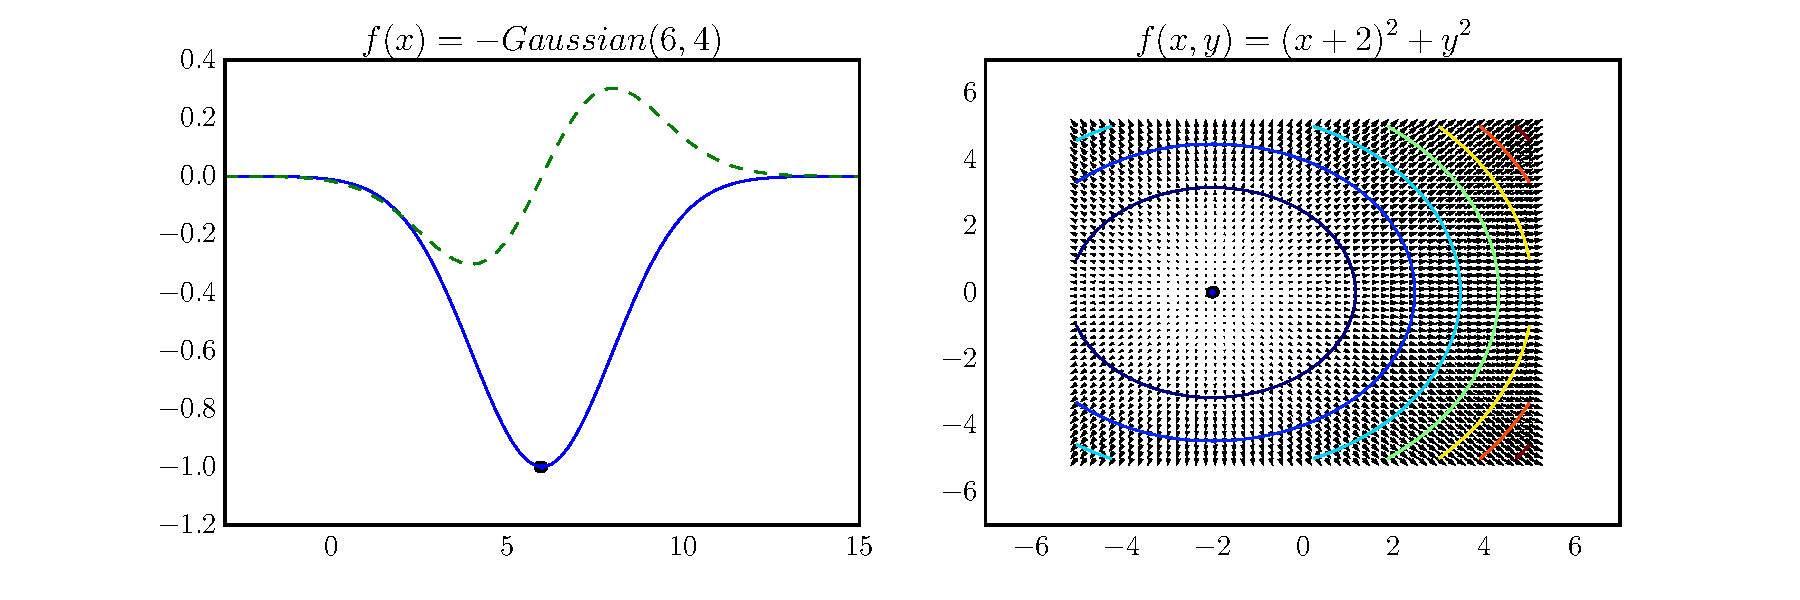
\includegraphics[width=.66\textwidth]{exercise1-2-ab.pdf}
	\caption{(a) Convex function with known minimum value and it's analytical derivative. The dots are the calculated minima according to gradient descent. (b) Contour plot of the gradient of a scalar function with vector-valued arguments. The dots are the calculated minima according to gradient descent.}
	\label{fig:1-2-ab}
\end{figure}

Figure \ref{fig:1-2-c} shows the result of using gradient descent on function (c) with different parameters. The sequence of dots in each case represents the guesses that gradient descent takes to be the minimum. In general, the choice of starting point affects which local minimum gradient descent will find. If the starting point chosen is a local maximum, the procedure will not step towards a minimum because the gradient is zero at the maximum. If the step size is large, the procedure will overshoot the minimum and zig-zag back to the desired minimum, taking a large number of iterations to converge. 

\begin{figure}[!ht]
	\centering
	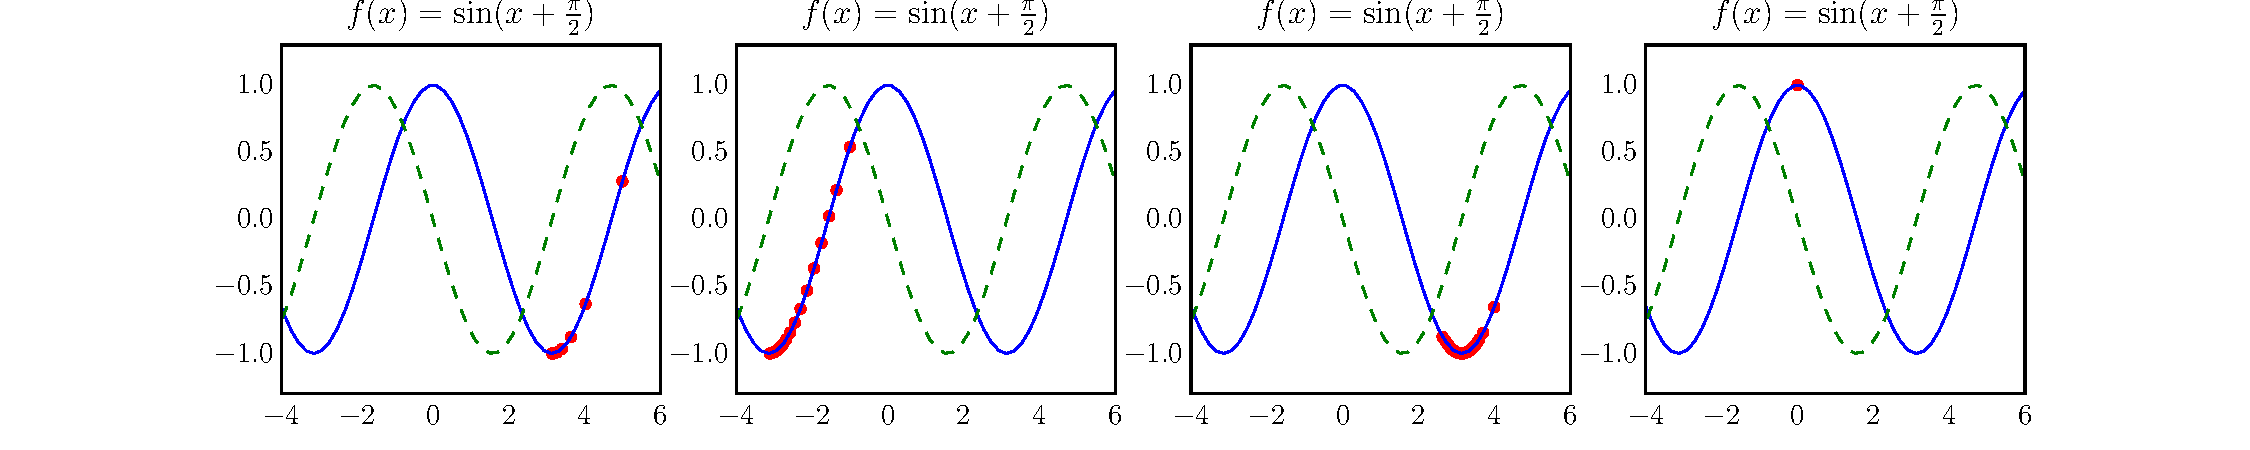
\includegraphics[width=\textwidth]{exercise1-2-c.pdf}
	\caption{The solid line is the function, the dashed line is its analytical derivative, and the series of dots is the series of minimum guesses from gradient descent. (a) Initial guess: 5, step: 0.5, threshold: 0.1 converges in 9 iterations. (b) Initial guess: -2, step: 0.2, threshold: 0.1 converges in 20 iterations. (c) Initial guess: 4, step: 2, threshold: 0.1 converges in 59992 iterations. (d) Initial guess: 0, step: 0.5, threshold: 0.1 converges in 1 iteration, but does not converge to a minimum. }
	\label{fig:1-2-c}
\end{figure}

Approximating a function's gradient using central differences is very accurate if using an $h$ of $1$. Figure \ref{fig:1-3-a} shows graphs of either the gradient function or gradient vector field for the three functions tested above. It is hard to tell the difference between the analytical and numerical functions, so using central differences to numerically estimate the gradient is effective.

\begin{figure}[!ht]
	\centering
	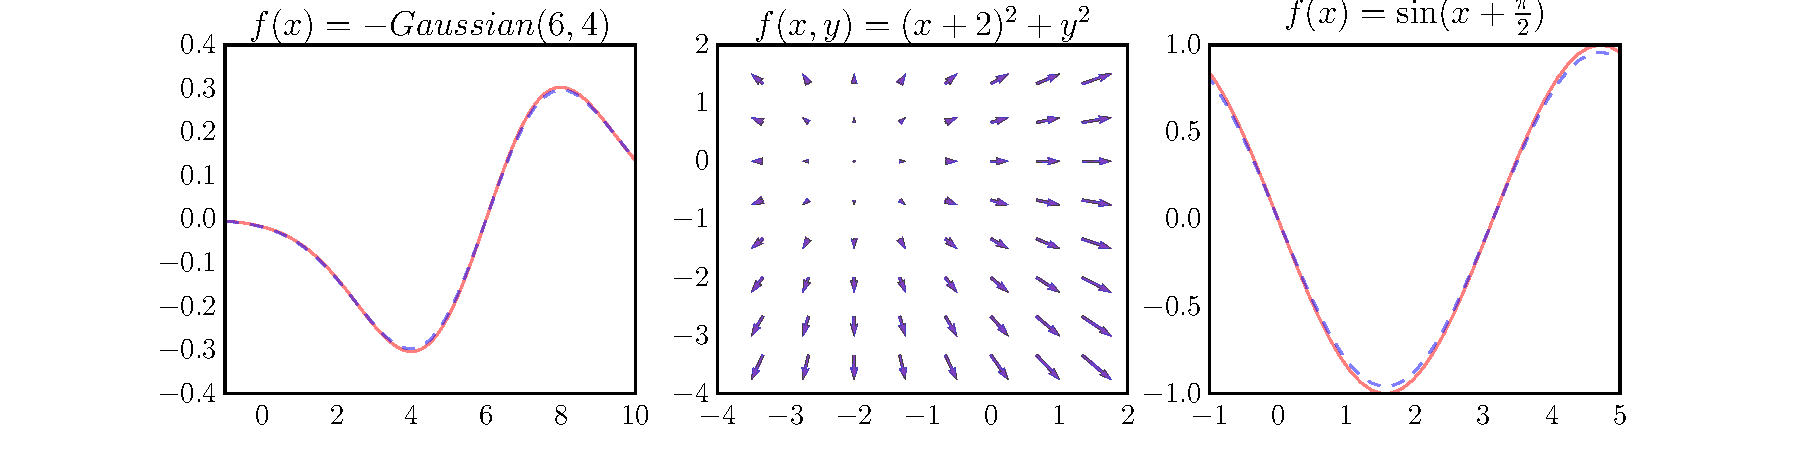
\includegraphics[width=\textwidth]{exercise1-3-a.pdf}
	\caption{The analytical and numerical gradients for the functions (a) upside-down Gaussian, (b) $f(x, y)= (x + 2)^2 + y^2$, and (c) $f(x) = \sin(x + \frac{\pi}{2})$. The solid red line is the analytical gradient and the dashed blue line is the numerical gradient.}
	\label{fig:1-3-a}
\end{figure}

The \textsc{BFGS} optimizer in SciPy uses a more sophisticated method for estimating minima, so in general, the number of function evaluations needed before convergence is smaller. Table \ref{tbl:1-4-a} shows a comparison of the gradient descent and \textsc{BFGS} optimizer, where in all cases the step size was $0.2$ and the threshold was $0.01$.

\begin{table}[!ht]
\centering
\makebox[\textwidth][c]{
\begin{tabular}[ht]{ccccc}
Function & Initial Guess & Algorithm & Evaluations & Min at\\\hline
\multirow{2}{*}{$f(x) = -$Gaussian$(6, 4)$} & \multirow{2}{*}{$x = 5$} & GD & 34 & $x = 5.81$ \\
 & & \textsc{BFGS} & 6 & $x = 6.00$ \\\hline
\multirow{2}{*}{$f(x, y) = (x + 2)^2 + y^2$} & \multirow{2}{*}{$(x, y) = (5, 5)$} & GD & 13 & $(x, y) = (-2, 0)$\\
 & & \textsc{BFGS} & 4 & $(x, y) = (-2, 0)$ \\\hline
\multirow{2}{*}{$f(x) = \sin(x + \frac{\pi}{2})$} & \multirow{2}{*}{$x = 5$} &  GD & 20 & $x = 3.15$ \\
 & &  \textsc{BFGS} & 6 & $x = 3.14$ \\
\end{tabular}
}
\caption{Steps to convergence given a similar set of parameters. GD is gradient descent, \textsc{BFGS} is from SciPy. For gradient descent, all step sizes were $0.5$ and thresholds were $0.01$.}
\label{tbl:1-4-a}
\end{table}

% \newpage
\section{Exercise 2}

\begin{figure}[!ht]
	\centering
	\makebox[\textwidth][c]{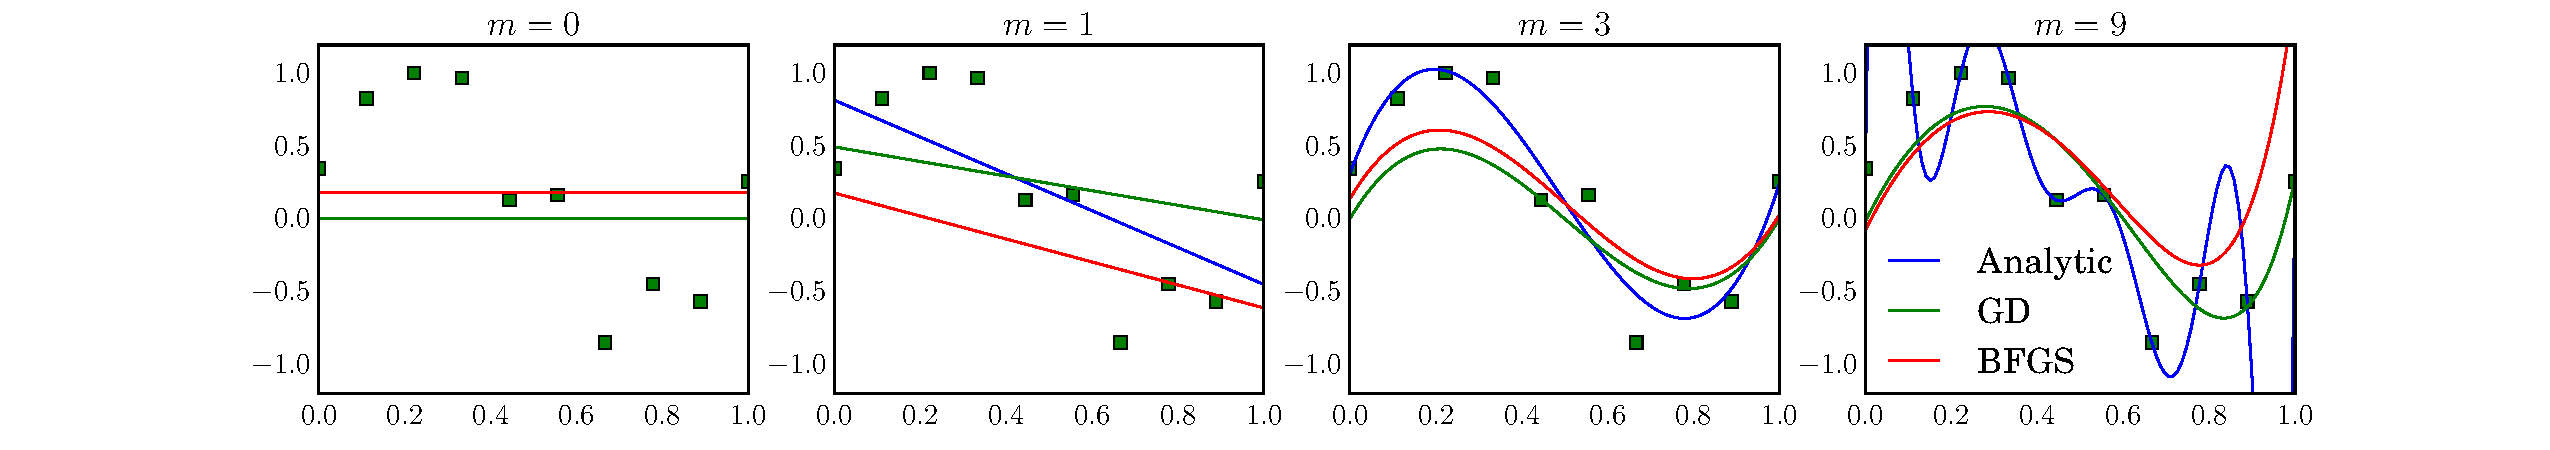
\includegraphics[width=1.25\textwidth]{exercise2-1.pdf}}
	\caption{Plots replicating Figure 1.4 in Bishop for different values of $M$ using different methods. The blue is generated with the analytical solution of the SSE, the green with the gradient descent method on the SSE, and the red using Python's \textsc{BFGS} optimizer.}
	\label{fig:2-1}
\end{figure}

\begin{figure}[!ht]
\centering
\makebox[\textwidth][c]{
\begin{subtable}[!ht]{0.38\textwidth}
\centering
\scalebox{0.8}{
\begin{tabular}{l|rrrr}
	& $M = 0$ & $M = 1$ & $M = 6$ & $M = 9$ \\\hline
	$\hat{w}_0$ & $0.186$ & $0.820$ & $0.353$ & $0.349$ \\
	$\hat{w}_1$ & & $-1.268$ & $2.619$ & $232.411$\\
	$\hat{w}_2$ & & & $32.096$ & $-5322.833$\\
	$\hat{w}_3$ & & & $-206.273$ & $48577.404$\\
	$\hat{w}_4$ & & & $399.001$ & $-231682.150$\\
	$\hat{w}_5$ & & & $-332.709$ & $640159.305$\\
	$\hat{w}_6$ & & & $105.163$ & $-1061992.54$\\
	$\hat{w}_7$ & & & & $1042586.68$ \\
	$\hat{w}_8$ & & & & $-557781.754$\\
	$\hat{w}_9$ & & & & $125223.393$\\
\end{tabular}
}
\end{subtable}
\hspace{2mm}
\begin{subtable}[!ht]{0.38\textwidth}
\centering
\scalebox{0.8}{
\begin{tabular}{l|rrrr}
	& $M = 0$ & $M = 1$ & $M = 6$ & $M = 9$ \\\hline
	$\hat{w}_0$ & $0.003$ & $0.499$ & $0.623$ & $-0.014$ \\
	$\hat{w}_1$ & & $-0.502$ & $5.577$ & $6.018$ \\
	$\hat{w}_2$ & & & $-14.465$ & $-12.820$ \\
	$\hat{w}_3$ & & & $5.502$ & $6.294$ \\
	$\hat{w}_4$ & & & $0.475$ & $-5.629$ \\
	$\hat{w}_5$ & & & $0.453$ & $4.425$ \\
	$\hat{w}_6$ & & & $0.435$ & $0.464$ \\
	$\hat{w}_7$ & & & & $0.493$ \\
	$\hat{w}_8$ & & & & $0.516$ \\
	$\hat{w}_9$ & & & & $0.533$ \\
\end{tabular}}
\end{subtable}
\hspace{-3mm}
\begin{subtable}[!ht]{0.38\textwidth}
\centering
\scalebox{0.8}{
\begin{tabular}{l|rrrr}
	& $M = 0$ & $M = 1$ & $M = 6$ & $M = 9$ \\\hline
	$\hat{w}_0$ & $0.186$& $0.181$ & $0.133$ & $-0.077$ \\
	$\hat{w}_1$ & & $-0.791$ & $4.974$ & $6.080$ \\
	$\hat{w}_2$ & & & $-0.150$ & $-12.746$ \\
	$\hat{w}_3$ & & & $4.964$ & $6.398$ \\
	$\hat{w}_4$ & & & $-0.027$ & $-5.494$ \\
	$\hat{w}_5$ & & & $-0.020$ & $4.586$ \\
	$\hat{w}_6$ & & & $-0.013$ & $0.646$ \\
	$\hat{w}_7$ & & & & $0.692$ \\
	$\hat{w}_8$ & & & & $0.729$ \\
	$\hat{w}_9$ & & & & $0.758$ \\
\end{tabular}}
\end{subtable}
}
\caption{Table 1.1 from Bishop replicated using (a) analytical solutions, (b) gradient descent, and (c) the Scipy \textsc{BFGS} optimizer}
\label{tbl:bishop-1-1}
\end{figure}

\begin{table}[!ht]
\centering
\makebox[\textwidth][c]{
\begin{tabular}{c|cccc}
& $M=0$ & $M=1$ & $M=3$ \\\hline
SSE & $3.774$ & $2.237$ & $0.350$\\\hline
$\nabla$ SSE analytic & $2.2\e{-16}$ & $(1.3\e{-15}, -1.3\e{-15})$ & $(-3.3\e{-14}, -6.4\e{-15},$ \\
& & & $ -5.8\e{-15}, -1.7\e{-14})$ \\\hline
$\nabla$ SSE numeric & $0$ & $(2.7\e{-15}, -1.3\e{-15})$ & $(-3.4\e{-14}, -6.2\e{-15},$\\
& & & $-7.7\e{-15}, -1.7\e{-14})$ \\
\end{tabular}
}
\caption{Values of the SSE and the analytical and numerical gradients for the given values of $M$ calculated using the $w$ coefficients calculated from the analytical solution.}
\label{tbl:sse}
\end{table}

There are three ways to calculate the maximum likelihood weight vector to minimize the $L2$ norm - (a) analytically with matrices, (b) using gradient descent, and (c), using Scipy's built-in optimizer. Figure \ref{fig:2-1} shows the plots from Bishop Figure 1.4 reconstructed using the analytical (blue), gradient descent (green), and Scipy \textsc{BFGS}  (red) methods for different values of $M$. The coefficients from all three methods for the different values of $M$ in Bishop's Table 1.1 are given in Table \ref{tbl:bishop-1-1}. In general, the analytic computation matched Figure 1.4 in Bishop very well.

The analytic function to compute the gradient of the SSE was compared against the numeric central difference method in Table \ref{tbl:sse}, using the weights computed by the analytic method for the various values of $M$. The methods match, so the analytic function is a valid one to use for further optimization.

When recreating Bishop's Figure 1.4 using gradient descent and the \textsc{BFGS}, the same initial guess was given, and the analytic formula of the SSE gradient was used, for simplicity and consistency. Choosing initial guesses, step sizes, and thresholds for gradient descent strongly influences the results. In general, the closer the initial guess is to the analytic solution, the more likely the gradient descent function will find it. This is because the gradient of the SSE has multiple zeros - if there is an optimization for $9$ weights, then the SSE function is degree $9$, which means it can at most have $4$ local minima, according to Euler's theorem. This means that as in the discussion of Exercise 1 above, the gradient descent function will find different minima according to the start value. The threshold and step size were chosen to be $0.001$ and $0.01$ respectively, so that the gradient descent function came as close to the analytic solutions without taking too long to compute. The \textsc{BFGS} optimizer behaved like the gradient descent minimizer, except no threshold or step size needed to be given. However, it was strongly influenced by the initial guess, as discussed above.

\section{Exercise 3}

\begin{figure}[!ht]
	\centering
	\makebox[\textwidth][c]{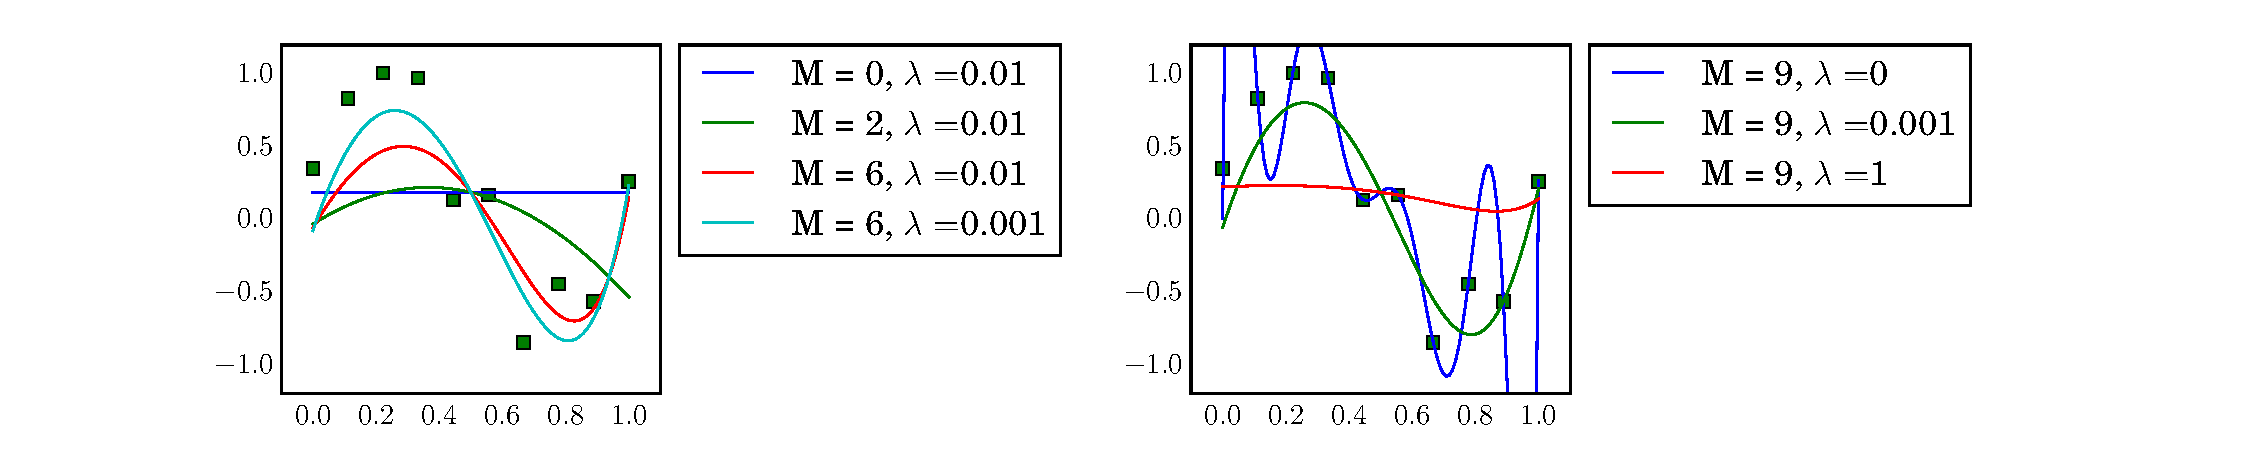
\includegraphics[width=1.25\textwidth]{exercise3-1.pdf}}
	\caption{Predicted regressions using ridge regression for various values of $M$ and $\lambda$}
	\label{fig:3-1}
\end{figure}

Figure \ref{fig:3-1} shows the plots of predicted regression values using ridge regression for various values of $M$ and $\lambda$. Because a value of $\lambda=0$ corresponds to no regularizer, the plot for $M=9$ looks like the plots from Exercise 2 above. As $\lambda$ increases to $1$ and greater for all values of $M$, the predicted regression becomes more flat, since the regularizer punishes having large coefficients. Small values of $\lambda$ that are not $0$ yield good results. There is no benefit to increasing $M$ after a certain point when regressing with a regularizer.

\begin{figure}[!ht]
	\centering
	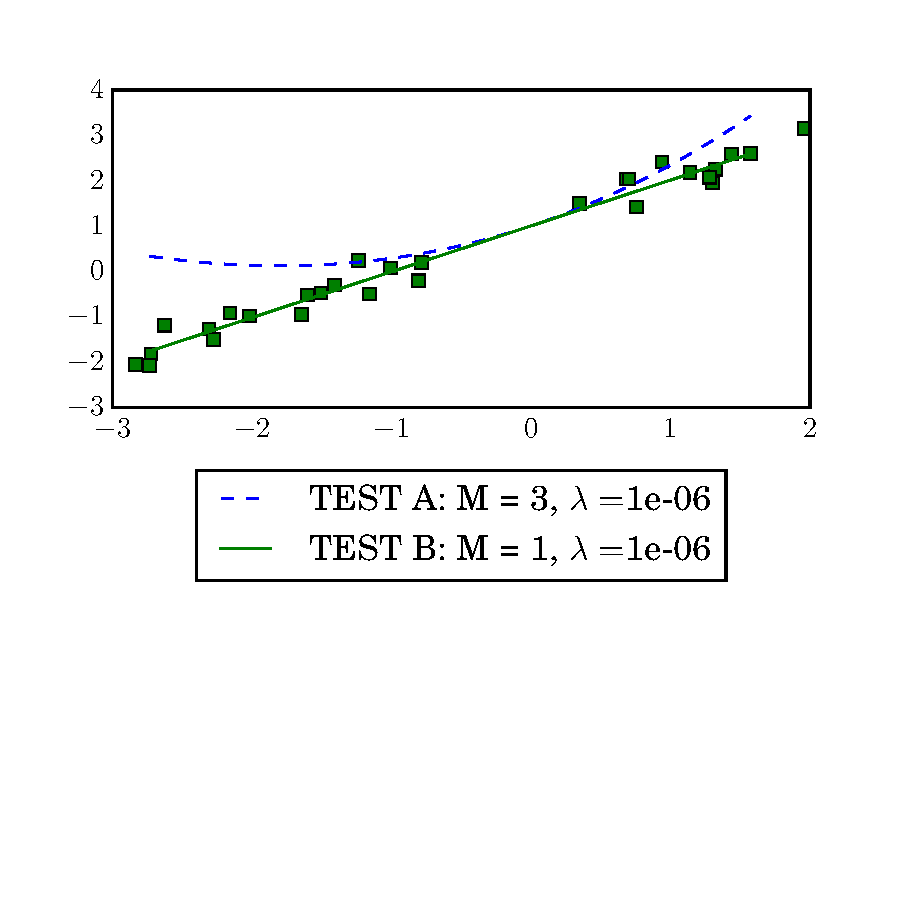
\includegraphics[width=\textwidth]{exercise3-2-1.pdf}
	\caption{The optimal regression lines for (a) Set A and (b) Set B and their corresponding $M$ and $\lambda$ values. (c) is a plot of all the data together (sets A and B as well as the training data)}
	\label{fig:3-2}
\end{figure}

There were two sets, A and B, in addition to a validation set given. To do model selection and test the results, I split each set A or B into two sets: half (arbitrarily the first half) became the training set, and half became the validation set (arbitrarily the second half). The validation set became the training set that the errors were reported on. To find the best regression, first choose an $M$ value using ridge regression with $\lambda = 0$ and iterating over all possible values of $M$ as there are data points. The $M$ that gives the smallest MSE for the training set, use that to test values of $\lambda$ that minimize the MSE on the validation set. The results of using set A as training vs. set B as training is given in Figure \ref{fig:3-2}. The SSE for set A on the test set is $0.91$ and the MSE for set B on the test set was $1.25$. The reason that set B gives a more complex model is that the data used in the training set was not uniformly distributed around the optimal regression line - the errors from the training set were pulling the model coefficients into higher complexity. In reality, neither model accurately describes all given data. This means that the choice of training data selection from the entire dataset strongly affects the regression output.

\begin{figure}[!ht]
	\begin{center}
	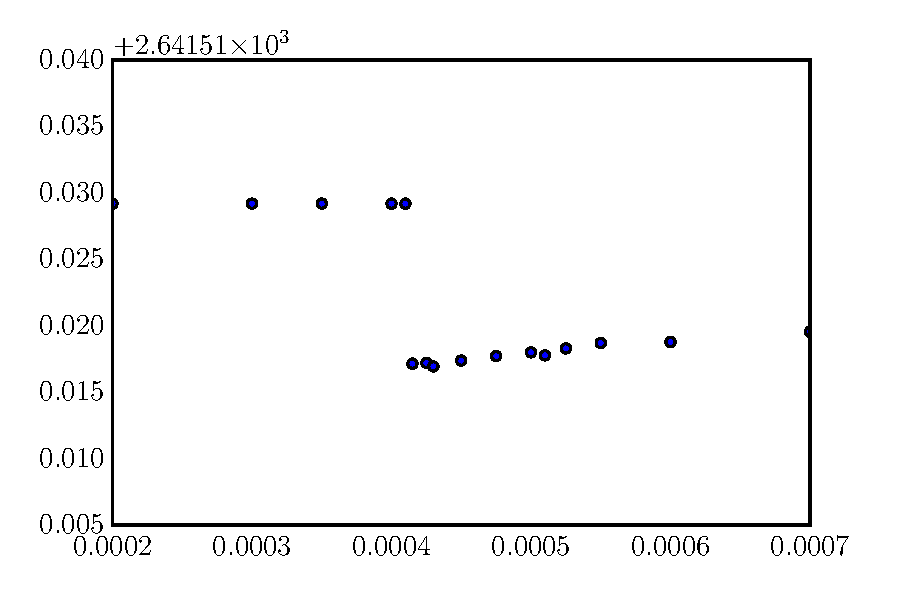
\includegraphics[width=0.48\textwidth]{exercise3-2-3.pdf}
	\caption{A plot of the MSE (mean square error) as a function of different values of $\lambda$}
	\label{fig:3-3}
	\end{center}
\end{figure}

For the blogset data, a similar procedure was used. The training data was used to select the model class $M$. Values of $M \neq 2$ with $\lambda = 0$ yielded singular matrices when solving for optimal $w$, so the model class was chosen as $M = 1$ (MSE for $M = 1, \lambda = 0$ on the training set was $880.597$). Then the validation set was used to find the optimal value of $\lambda$. At the optimal value of $\lambda$ for $M = 1$ on the validation set, the MSE was $2641.527$. Figure \ref{fig:3-3} shows a plot of the MSE as a function of $\lambda$ for $M = 1$. With the optimal value of $\lambda$ chosen as the inflection point of the graph, the optimal parameters and test MSE were found to be $M = 1, \lambda = 0.00043,$ MSE = $2641.527$. 

\section{Exercise 4}

\begin{figure}[!ht]
	\begin{center}
	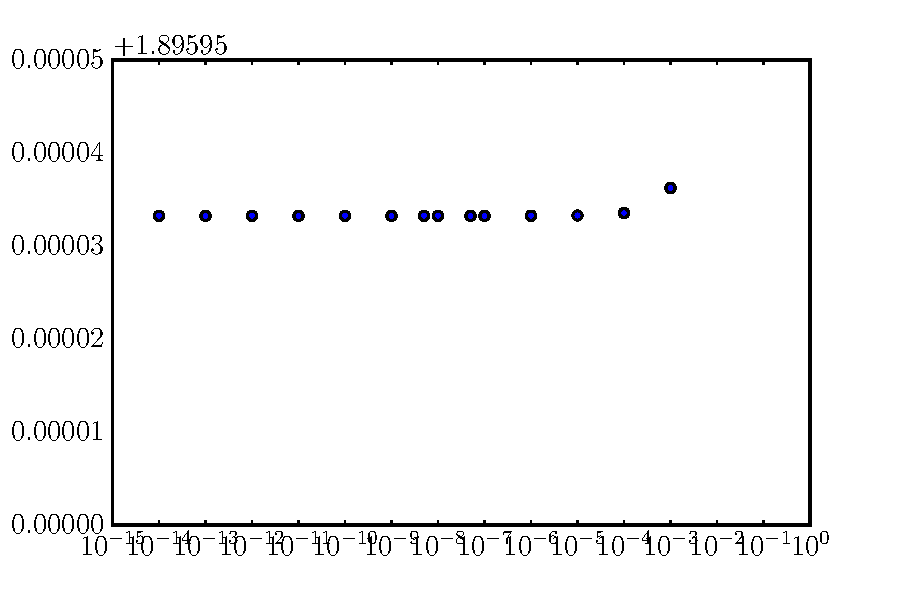
\includegraphics[width=0.48\textwidth]{exercise4-1.pdf}
	\caption{A plot of the LAD (least absolute deviation) as a function of different values of $\lambda$ for $M = 1$. The x-values are on a log scale.}
	\label{fig:4-1}
	\end{center}
\end{figure}

For the LAD, repeating the experiments from Exercise 3 with central differences is difficult because the derivative of the LAD is discontinuous. Therefore, the gradient descent function goes through thousands of iterations and sometimes does not converge. My solution for mitigating this problem was to stop the gradient descent function after 2000 iterations, and the start value of the values of $w$ was always a list of zeros. Even when given a start value of $(-1, 1)$, which is close to the `optimal' solution, the LAD does not perform well. The same algorithm as in Exercise 3 was then applied - the training dataset (set A) was used to select the optimum value of $M$ when $\lambda = 0$, which was determined to be $M = 1$. Then set B was the validation set that was used to find the optimum value of $\lambda$ when $M = 1$, searched for with a binary-like search. When calculating $M$, the step size for gradient descent was $0.001$ and the threshold was $0.0001$, which yielded good results. To get more accurate coefficients and a finer-grained search during $\lambda$ selection, a step size of $0.00005$ and threshold of $0.00001$ were used. For the $\lambda$ selection, the  Figure \ref{fig:4-1} shows a plot of log-$\lambda$ vs LAD error. The optimal value of $\lambda$ was found to be $1\e-13$. Then the given validation set became the test set, where the LAD error was found to be $1.654$. One thing to watch out for when using gradient descent is that the threshold and the step size have an effect on the optimal value of $\lambda$ - the smaller the threshold, the smaller the optimal value of $\lambda$. 

\begin{figure}[!ht]
	\begin{center}
	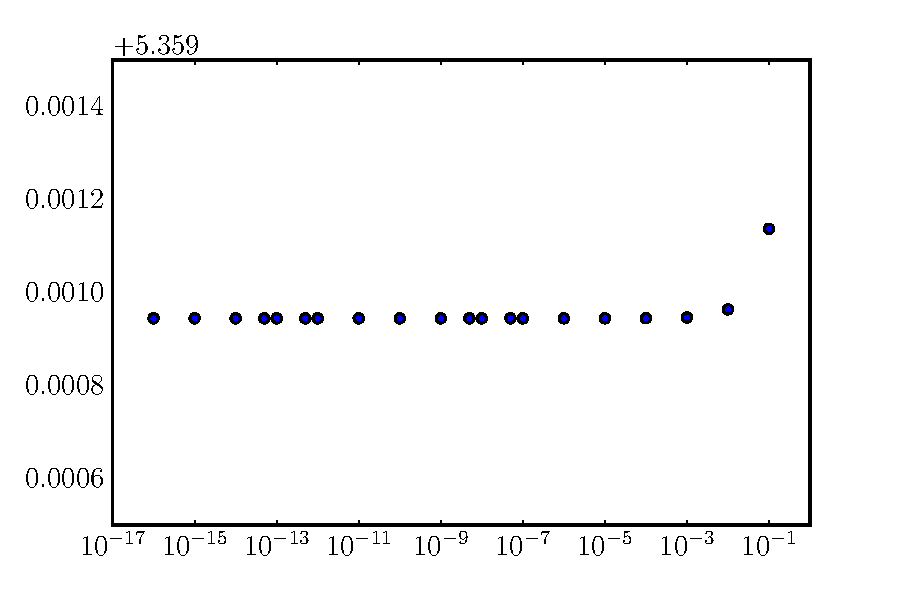
\includegraphics[width=0.48\textwidth]{exercise4-2.pdf}
	\caption{A plot of the Lasso as a function of different values of $\lambda$ for $M = 1$. The x-values are on a log scale.}
	\label{fig:4-2}
	\end{center}
\end{figure}

When optimizing with gradient descent on a lasso with least-squares error, the same method was used as described above for LAD, including the limiting of computation time on the gradient descent. In choosing $M$, the error grows very quickly with increasing values of $M$ if the start value is all zeros in the gradient descent, so the start value was changed to $(-1, 1)$. The optimal $M$ chosen was $M = 1$. On set B, the optimal value of $\lambda$ was calculated to be $1\e-10$. Figure \ref{fig:4-2} is a plot of the Lasso error as a function of $\lambda$ for $M = 1$. The error on the test set was $0.056$. In the Lasso case, the choice of step size, starting value, and threshold less strongly affect the optimal value of $\lambda$ and the value of the error. 

In both cases of LAD and Lasso, the starting value, step size, and threshold have an enormous effect on the outcome of the optimization. However, in my experiments, the Lasso was much more sensitive to start values.

It is wise to use Lasso as an estimator when there are a lot of features, since the constraints on the Lasso penalize having many variables, therefore decreasing model complexity. In both cases, loss function that is presented in the problem becomes the error function used to measure success of the predictive model. So in the case of an absolute value loss $L(p, a) = |p - a|$, the LAD approach is the correct measure of success, since it is the same measure of loss. For all approaches to measuring model success, the given loss function must match the error function. 

\end{document}